\sloppy

\section{Introduction}

For samples of star forming galaxies in the local and high redshift Universe there is a well observed correlation between the far-infrared and radio emission (e.g. \citealt{Dickey_1984, deJong_1985, Helou_1985, Condon_1992, Barger_2000, Yun_2001, Garrett_2002, Appleton_2004, Ibar_2008, Seymour_2009, Sargent_2010}), that remains nearly linear over multiple orders of magnitude in far-infrared luminosity ($10^{9} \lesssim L_{\textrm{FIR}} [L_{\odot}] \lesssim 10^{12.5}$). The small scatter in this relation is often attributed to the \textit{calorimeter model} (\citealt{Voelk_1989, Lisenfeld_1996, Lacki_2010}), which ascribes the far-infrared and radio emission to common stellar sources. In this model, galaxies are opaque to UV light from massive OB-like stars which gets absorbed by the dust in the ISM and reradiated in the far-infrared. Observations in the far-infrared and sub-mm are thus sensitive to the cold dust that reradiates the energy from young stars. These stars quickly come to the end of their lives, exploding as Type II supernovae, producing cosmic ray electrons and positrons. These cosmic rays are emitted with relativistic velocities that radiate energy in the radio as synchrotron radiation when spiralling around galactic magnetic fields. The concurrence of the far-IR and radio emission in a galaxy means that the radio continuum is a useful tracer of recent, obscured star formation.

The prevalence of a correlation at such a wide span of redshifts and luminosities has lead to studies that use the radio emission as an unbiased tracer of obscured star formation in dusty galaxies across time (\citealt{Kennicutt_2012}). {\color{red}AGN here}

By making use of the tight far-IR/radio correlation (FIRC), as well as the benefits we shall outline in the following section, we can identify counterparts to low resolution sources with greater confidence than we would expect if we directly matched to the optical or near-infrared, which allows for better characterization of the galaxies' properties. In this Chapter, we identify $3\,$GHz VLA counterparts to \textit{Herschel} detected galaxies in the $\sim2\,$deg$^2$ COSMOS field. The radio galaxies themselves have short wavelength counterparts provided by the COSMOS2020 catalogue, that we match unambiguously due to their much smaller positional errors.

\section{Identifying Multiwavelength Counterparts to DSFGs via the Radio}

As illustrated in Chapter \ref{chapter:Data_Release_3}, DSFGs that are detected with single dish far-IR/sub-mm telescopes with low angular resolution will likely include multiple galaxies in the optical or near-infrared within the beam width. This is a particular problem for \textit{Herschel} where even the smallest SPIRE beam size, at $250\,\mu$m, has a FWHM of $\sim 18\,$arcsec, making the decision as to the source of the far-IR emission difficult. This is further compounded by the intrinsic faintness of optical counterparts due to dust obscuration. In the following sections we detail a method for identifying radio counterparts to \textit{Herschel} sources, that makes use of the FIRC to identify them with high confidence. This circumvents the uncertainty that comes from statistical methods that match directly to short wavelength counterparts by first matching them with radio sources that have small positional errors, thus generating a clean and more complete sample. The following is a list of benefits of using the radio emission for this purpose:

\begin{enumerate}
    \item Star forming galaxies are known to produce a lot of synchrotron emission. This allows us to take advantage of the FIRC to locate the galaxy emitting the radiation in the far-IR. Unlike optical counterpart searches, radio IDs are not solely motivated by their position and brightness, but also by the fact that the two regimes are linked to a common source.
    \item Even when considering the deepest radio maps, the low surface density of radio sources means that the probability of a chance positional alignment is unlikely. As a result, we can have a reasonable confidence in there being some association between objects when we do observe radio sources in close proximity to the far-IR/sub-mm position (\citealt{Ivison_2002, Borys_2004}). In most cases (as we shall validate in this study), radio sources are sufficiently rare that finding an object within the positional uncertainty of the far-IR/sub-mm beam almost always results in a secure identification.
    \item When a secure radio counterpart is identified, the positional accuracy ($\sim 1\,$arcsec for the Karl G. Jansky Very Large Array (VLA) at $1.4\,$GHz and $\sim 0.75\,$arcsec at $3\,$GHz) allows for an unambiguous identification with an optical or infrared galaxy counterpart. By first locating these galaxies via their radio identification, we predict a low false identification rate which gives us greater confidence in characterizing their colours, morphologies, stellar masses and more.
\end{enumerate}

While the radio emission from star forming galaxies allows for more secure identification of counterparts across the electromagnetic spectrum, it also has several drawbacks. The following is a list of disadvantages to using radio emission for this purpose:

\begin{enumerate}
    \item Our understanding of the radio-selected DSFG population is likely to be skewed by selection effects. The negative K-correction in the far-infrared arises due to the steep Rayleigh-Jeans part of the SED and allows for nearly equal detection of dusty galaxies at $z \sim 0.5$ as $z \sim 8$ (\citealt{Blain_2002}). The radio, however, suffers from a strong positive K-correction which causes a bias against high redshift galaxies ($z > 3$). This means that a substantial fraction of far-IR and sub-mm detected galaxies remain undetected in the radio due to the lack of sufficiently deep radio data.
    %\item Long wavelength interferometry has been used to show that for far-IR/sub-mm sources in which we observe multiple radio galaxies in close proximity, in $\sim 80\%$ of cases the thermal dust emission is associated from only one of the radio sources. This leads to an ambiguity as to the nature of some apparent multiple systems. This will be discussed in more detail in Section \ref{sec:multiple_systems}.
    \item {\color{red}AGN here}
	\item Potentially the most important drawback for the identification of far-IR/sub-mm emitting galaxies, is the sky coverage from radio surveys. While we have large sky surveys in the far-IR such as \textit{Herschel}-ATLAS, using deep radio data for such large areas is not yet practical. The capabilities of future radio surveys such as the Square Kilometre Array (SKA) and recent wide-area surveys with the Low-Frequency Array (LOFAR) will allow us to produce larger samples of DSFGs.
\end{enumerate}

Many studies have found success in adopting a frequentist approach to identifying radio counterparts to far-IR/sub-mm sources (e.g. \citealt{Eales_2009, Dye_2009, Dunlop_2010} and references therein). This typically involves using Monte Carlo simulations to estimate the probability that a given radio source is located near the far-IR/sub-mm position by chance. This is in contrast to the Likelihood Ratio method described in Chapter \ref{chapter:Data_Release_3} where we defined a probability of association for each possible counterpart. With the lower surface density of radio objects on the sky, a better question to ask ourselves is: how many ways would we expect to observe a given candidate by chance? This naturally lends itself to using a Monte Carlo approach. The advantage of using such a frequentist approach over a Bayesian method is that it does not require assumptions to be made about the form of the far-IR/sub-mm positional errors, given that they are poorly known due to source confusion. {\color{red}Consider adding more about why the LR method is not used here.}

\section{Identifying Radio IDs to \textit{Herschel} Sources in COSMOS}

In the following sections we identify radio counterparts to \textit{Herschel} detected sources in the Cosmic Evolution Survey (COSMOS), applying the frequentist method of \citealt{Lilly_1999}. COSMOS is a deep, wide area survey of an equatorial two square degree field centered at R.A $+150.12^{\circ}$ and declination $+2.21^{\circ}$ (\citealt{Scoville_2007}). The field has been observed with many space-based (e.g. \textit{Hubble Space Telescope}, \textit{Spitzer}, \textit{Chandra} and \textit{Herschel}) and ground-based telescopes (e.g. Keck, VLA and UKIRT), resulting in multiwavelength data that spans from the X-ray to radio wavelengths. The high sensitivity and resolution of these data sets over a sufficiently large area, allows for comprehensive studies on the co-evolution of galaxies (\citealt{Schreiber_2018}; \citealt{Stockmann_2020}; \citealt{Valentino_2020a}), star formation (\citealt{Gruppioni_2013}; \citealt{Novak_2017}), large scale structure (\citealt{Scoville_2013}; \citealt{Laigle_2018}) and AGN (\citealt{Prescott_2006}; \citealt{Heintz_2016}). 

\subsection{\textit{Herschel} Observations in COMSOS}

The \textit{Herschel} detected sources that we study in this work were taken as part of the \textit{Herschel} Multi-tiered Extragalactic Survey (HerMES; \citealt{Oliver_2012}). HerMES is a deep far-infrared imaging survey of some of the most well-studied blank extragalactic fields. The survey design of HerMES allowed for the detection of a wide range in far-IR luminosities by targeting high luminosity objects which are bright but rare in wide, shallow surveys and the lower luminosity objects, which are faint but common, in deep, narrow surveys. As such, fields range in size from $0.01$ to $\sim 20\,$deg$^2$. As part of the survey, the COSMOS field was observed with SPIRE over the full two square degrees. We take as our \textit{Herschel} catalogue, the $11,185$ SPIRE sources that were observed in the COSMOS field. {\color{red}Explain how the Herschel catalogue was formed.}

\subsection{VLA Observations in COSMOS}

The VLA-COSMOS $3\,$GHz Large Project (\citealt{Smolcic_2017a, Smolcic_2017b, Smolcic_2017c}) was a radio continuum survey covering $2.6\,$deg$^{2}$, enclosing the two square degrees of the COSMOS field, with a mean r.m.s sensitivity of $\sim 2.4\,\mu$Jy beam$^{-1}$ and an exceptional angular resolution of $0.75\,$arcsec at $3\,$GHz. Observations of the COSMOS field were taken in the S-band ($2 - 4\,$GHz) for a total of $384\,$hours. The large effective bandwidth ($\sim 2\,$GHz) and large field of view of the S-band allowed for fast coverage of COSMOS. The survey recovered $10,899$ radio source components with a significance greater than $5\sigma$. After combining multicomponent sources, we are left with a total of $10,830$ $3\,$GHz sources. The VLA-COSMOS $3\,$GHz catalogue builds on the existing $1.4\,$GHz VLA catalogue (VLA-COSMOS Large and VLA-COSMOS Deep projects: \citealt{Schinnerer_2004, Schinnerer_2007, Schinnerer_2010}) of $2,865$ $1.4\,$GHz-detected (L-band) radio sources. The increased sensitivity of the S-band compared to the L-band allows for a factor approximately four increase in the number of detected sources over a similar sky area (though we note that the sources detected in the $3\,$GHz catalogue are typically fainter).

\subsection{\textit{Herschel}, VLA and the COSMOS2020 Catalogue}

The sample that we use for our study are the \textit{Herschel}-detected galaxies from HerMES and the VLA-detected sources from the VLA-COSMOS $3\,$GHz Large Project, that define an overlapping region, as shown in Figure \ref{fig:sky_map}. This square region covers R.A  $+149.29^{\circ}$ to $+150.95^{\circ}$ and declination $+1.45^{\circ}$ to $+3.04^{\circ}$. This field spans a total area of $2.64\,$deg$^2$ and contains $7,230$ ($\sim 65\%$) \textit{Herschel} sources and $10,826$ ($\sim 100\%$) radio sources.

\begin{figure}
	\centering
	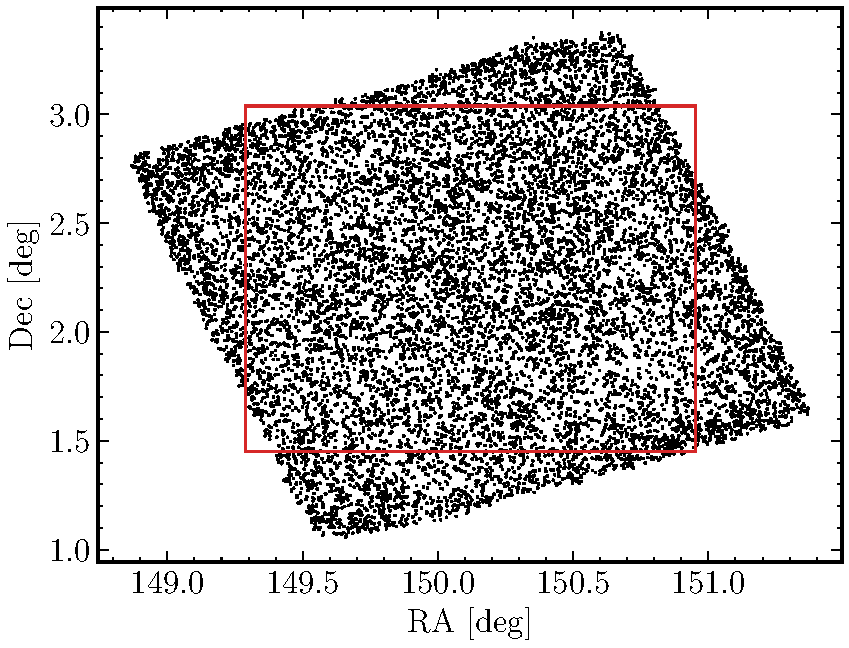
\includegraphics[width=0.8\columnwidth]{Figures/sky_map.pdf}
	\caption[Map of the \textit{Herschel} and VLA observations in the COSMOS field]{The map of \textit{Herschel} detections (black points) and the area covered by the VLA observations (red square). There are a total of $11,185$ \textit{Herschel} sources, of which $7,230$ ($64.6$\%) lie within the region covered by the VLA-COSMOS $3\,$GHz Large Project.}
	\label{fig:sky_map}
\end{figure}

The VLA-COSMOS $3\,$GHz Large Project is the deepest radio continuum survey that covers a field as large as that of COSMOS. Combined with the extensive multiwavelength data described above, it is a unique survey for studying the composition of the radio-detected galaxy population. As we shall explore later, the \textit{Herschel} sources with secure radio identifications in COSMOS make for an unparalleled set of far-IR selected galaxies that, with the wealth of data in the COSMOS field, have coverage across the electromagnetic spectrum. Such a sample would provide an excellent opportunity to precisely determine the galactic environments conducive to their high star formation rates and their evolution, and would also allow us to make predictions about the star forming galaxy populations in future radio surveys. These secure radio IDs will help facilitate the identification of dusty galaxies in large surveys from the likes of the SKA (\citealt{Dewdney_2009}) and the Next Generation Very Large Array (ngVLA), as well as their precursors such as the Australian Square Kilometre Array Pathfinder (ASKAP: \citealt{Johnston_2007}), the \textit{enhanced} Multi Element Remotely Linked Interferometer Network (\textit{e}-MERLIN), LOFAR and MeerKAT (\citealt{Jonas_2009}).

The wealth of imaging data for our \textit{Herschel} galaxies will come from the COSMOS2020 photometric redshift catalogue (\citealt{Weaver_2022}). This catalogue contains more than $1.7\,$million sources with UV to IR coverage. The positions of each source are based on a Gaia reference (\citealt{Gaia_2016}), which we match to a maximum separation of $0.5\,$arcsec with the $3\,$GHz positions. A total of $8,987$ ($83\%$) radio sources in COSMOS have short wavelength photometry.

\subsection{Calculating the Significance of Radio Associations}
\label{sec:radio_significance}

To predict the probability that an observed \textit{Herschel}-VLA pair are associated, we could use the Poisson probability detailed in \citealt{Downes_1986}. This defines the probability that a radio source of a given flux density could lie at the observed distance from the source by chance, and is given by $P = 1-e^{-\mu}$ where $\mu = \pi r^2n$. Here $r$ is the radial offset between the source and radio counterpart and $n$ is the surface density of objects brighter than the radio counterpart. While a low value of $P$ does not confirm that the radio object is the source of the emission, it does suggest that the two are likely associated. Obtaining a low value of $P$ can actually be interpreted in several ways. Firstly, the radio source could be the one true counterpart of the far-IR/sub-mm source. Second, the counterpart could be one of a group of galaxies that collectively contribute to the flux that is observed by \textit{Herschel}. Third, the low value of $P$ might represent an indirect association with the \textit{Herschel} source, for example, due to galaxy clustering with the true identification or a result of gravitational lensing.

In this study we use the method of \citealt{Lilly_1999}, which applies the same principles as the Poisson probability - that the probability of dissociation can be estimated from the distance from the source and the counterpart's flux density - but from a Monte Carlo perspective. The method, which is described in detail in \citealt{Dye_2009}, is as follows. First, we generate a set of $N$ random positions in the area common to both the \textit{Herschel} and radio surveys. Next, we identify all radio sources within some maximum radius, $r_{\textrm{max}}$, from each random position and measure the quantity $S = r^2n$, where $r$ and $n$ take the same definitions as earlier. Next, we take the minimum value of $S$ for each source (if there is more than one observable radio candidate, this corresponds to the most significant association) and use it to create a distribution of $S$, which we shall name in the same way as \citealt{Dye_2009}, $D(S)$. Much like the $K_s$-band magnitude distribution of background VIKING objects we derived in Chapter \ref{chapter:Data_Release_3}, $D(S)$ represents the distribution of $S$ values for random chance alignments. This distribution allows us to determine the probability of a radio source with $S = S_i$, observed within the search radius of a \textit{Herschel} position, being a random interloper. This is given by

\begin{equation}
    P(< S_i) = \frac{1}{N}\int_0^{S_i}D(S) dS.
    \label{eq:probability_frequentist}
\end{equation}

As is often assumed, we consider a radio source to be a secure identification if it has $P < 0.05$, suggesting that there is less than a $5\%$ probability that such a radio source would be observed by chance (e.g. \citealt{Ivison_2002, Ivison_2005, Pope_2006}). It is important to note that, depending on the surface density of radio galaxies, the maximum value of $P$ will often be less than one as some fraction of the randomly located positions will not contain any radio sources within $r_{\textrm{max}}$. 

The value of $r_{\textrm{max}}$ is an important choice. While a smaller search radius reduces the number of potential IDs and increases the likelihood of missing a true counterpart, a larger radius causes a greater probability of observing a background object and thus matching the source with an unrelated radio galaxy. A further complication is that too large a search radius causes overlapping fields which could lead to radio sources being connected to more than one \textit{Herschel} position. Some definitions for $r_{\textrm{max}}$ are based on a probabilistic balance of these two competing effects (e.g. \citealt{Dye_2009}), finding the radius where the expected number of false counterparts in the final sample equals the expected number of true identifications that are missed. In this study our aim is to define a clean sample of radio matched \textit{Herschel} sources, such that our multiwavelength photometry gives the most complete and accurate representation of our dusty galaxies. As we shall show later, this sample could provide a useful starting point for identifying dust enshrouded galaxies from future large area blank surveys (e.g. \textit{Euclid}). For this reason, we are less interested in ensuring the appropriate size of the sample, but rather in minimizing the number of falsely identified counterparts.

Figure \ref{fig:optimal_radius} shows the radial separation between the $7,230$ \textit{Herschel} positions and the VLA sources. We also plot the separation between $7,230$ random positions and the VLA sources, which follows a linear function in $r$. The peak at small $r$ shows the excess of counterparts over the background level, which contains our true identifications. The two distributions are equal at approximately $10\,$arcsec, which may seem like a search radius prone to misidentification, but if we consider the cumulative number of candidates out to a radius $r$ (inset figure), then we see that this radius corresponds to a maximum in the difference between the $\textit{Herschel}$ source distribution and the background distribution. This implies that at $\sim 10\,$arcsec the number of counterparts observed within the radius will be dominated by associated objects, which will aid in reducing the false identification rate. We adopt $r_{\textrm{max}} = 10\,$arcsec in this work.

\begin{figure}
	\centering
	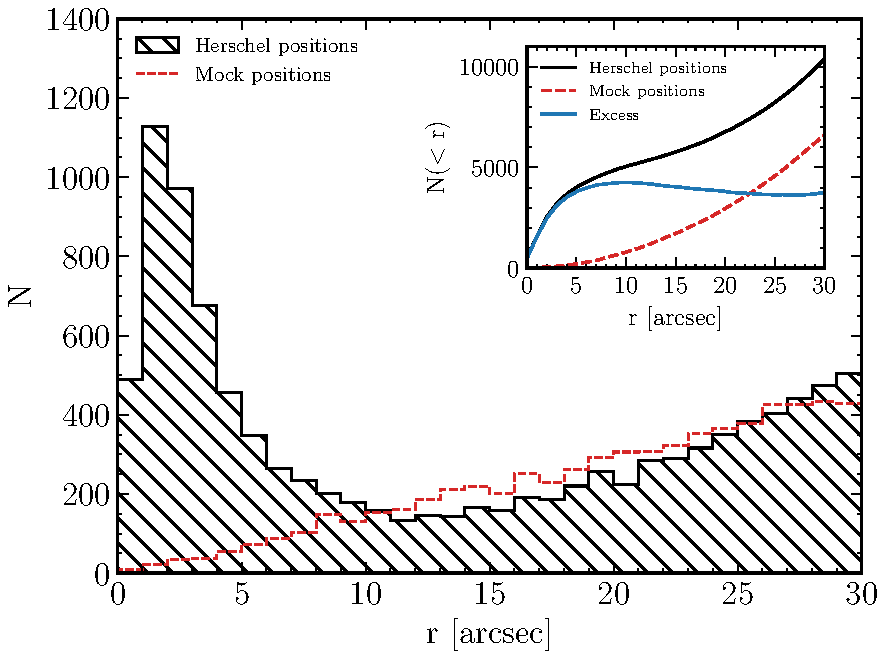
\includegraphics[width=0.8\columnwidth]{Figures/optimal_radius.pdf}
	\caption[Distribution of radial offsets between \textit{Herschel} sources and radio objects]{The distribution of radial offsets between \textit{Herschel} sources and radio candidates (black hatched histogram) and between random positions and radio candidates in the COSMOS field (red dashed line). The inset panel shows the cumulative distributions for the two histograms and the difference between them (blue solid line). The excess number of radio sources above the background level decreases beyond $\sim10\,$arcsec, we therefore choose $r = 10\,$arcsec as our maximum search radius.}
	\label{fig:optimal_radius}
\end{figure}

Given that our VLA observations have a surface density of $4,103\,$deg$^{-2}$ and we assume a fixed search radius of $10\,$arcsec, we can approximate the maximum value of $P$. As a first order approximation, the maximum $P$ value is equal to the ratio between the probability of observing at least one VLA source within $10\,$arcsec of a random position and the probability that the position is a blank field. Assuming Poisson statistics with a mean number of candidates per random position of $\lambda = N_{\textrm{VLA}}A_{\textrm{random}}/A_{\textrm{survey}}$, where $N_{\textrm{VLA}}$ is the number of VLA sources, $A_{\textrm{random}}$ is the search area around a single random position and $A_{\textrm{survey}}$ is the total survey area, then an estimate of $P_{\textrm{max}}$ can be given by

\begin{equation}
    P_{\textrm{max}} \approx \frac{P(\textrm{Not Blank})}{P(\textrm{Blank})} = \frac{P(X > 0)}{P(X = 0)} = \frac{1 - P(X = 0)}{P(X = 0)} = \frac{1 - e^{-\lambda}}{e^{-\lambda}} \approx 0.10,
\end{equation}

\noindent where $X$ is the number of VLA sources observed around each random position. This calculation suggests that the maximum $P$ value for any radio counterpart observed near a \textit{Herschel} source is $0.1$ (not considering effects such as clustering, multicomponent galaxies or overlapping search areas). The fact that only $\sim 10\%$ of random positions will be incident with at least one radio source gives further confidence in the association between any \textit{Herschel} and VLA sources found in close proximity.

\section{Results of the Monte Carlo Method Applied to \textit{Herschel} Sources}

We apply the method described above to all possible VLA counterparts within $10\,$arcsec of a \textit{Herschel} source. We retain all counterparts that have $P < 0.05$, but consider as our primary counterparts those with the lowest $P$ value per source. Figure \ref{fig:ds_distributions} shows the distribution of log($S$) for radio counterparts to \textit{Herschel} sources (black histogram) and $10^6$ random positions (red histogram). The clear offset between the two illustrates how a large fraction of the counterparts identified in the radio trace the dust emission.

\begin{figure}
	\centering
	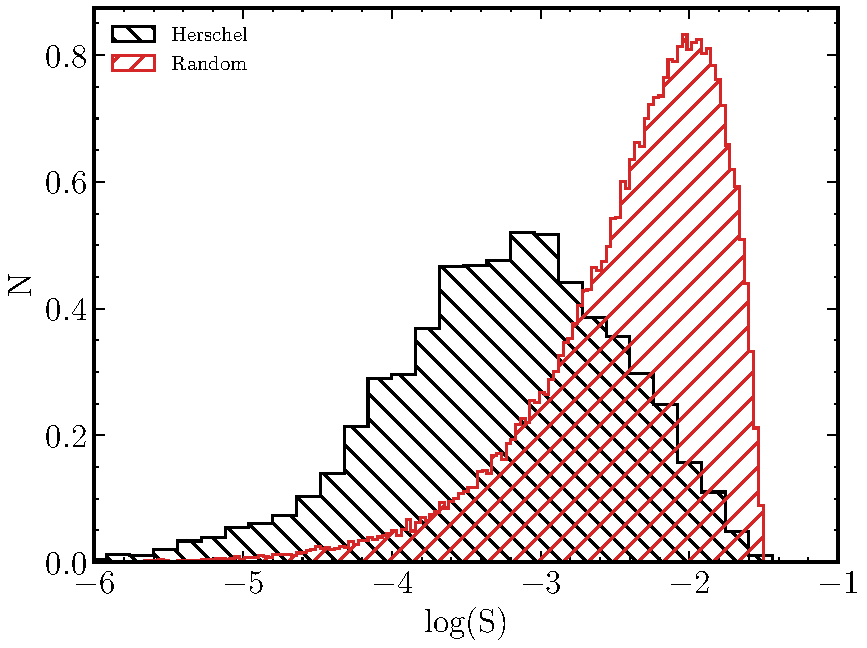
\includegraphics[width=0.8\columnwidth]{Figures/ds_distributions.pdf}
	\caption[Distribution of $\textrm{log}(S)$ for \textit{Herschel} sources and random positions]{The distribution of $\textrm{log}(S)$, as defined in Section \ref{sec:radio_significance}, for the most likely counterpart lying within $10\,$arcsec of the position of a \textit{Herschel} source (black histogram) and a random position (red histogram). The offset between the two distributions highlights the fact that many radio counterparts with low $S$ are truly associated with the \textit{Herschel} source.}
	\label{fig:ds_distributions}
\end{figure}

The total identification rate, that is the number of sources recovered with a $P < 0.05$ radio source, is $3,787$ ($52\%$). However, this is a strong function of the $250\,\mu$m flux density (Figure \ref{fig:id_rate}) and we observe a steep decline toward fainter $250\,\mu$m flux densities ($< 30\,$mJy) where we approach the confusion limit of the survey. From this point we refer only to the sources with $250\,\mu$m flux densities greater than 30\,mJy, where we are more confident that they correspond to real objects. In this case, the survey area corresponds to $1,324$ \textit{Herschel} sources with $S_{250} > 30\,$mJy, of which $1,053$ ($80\%$) have radio IDs with $P < 0.05$.

\begin{figure}
	\centering
	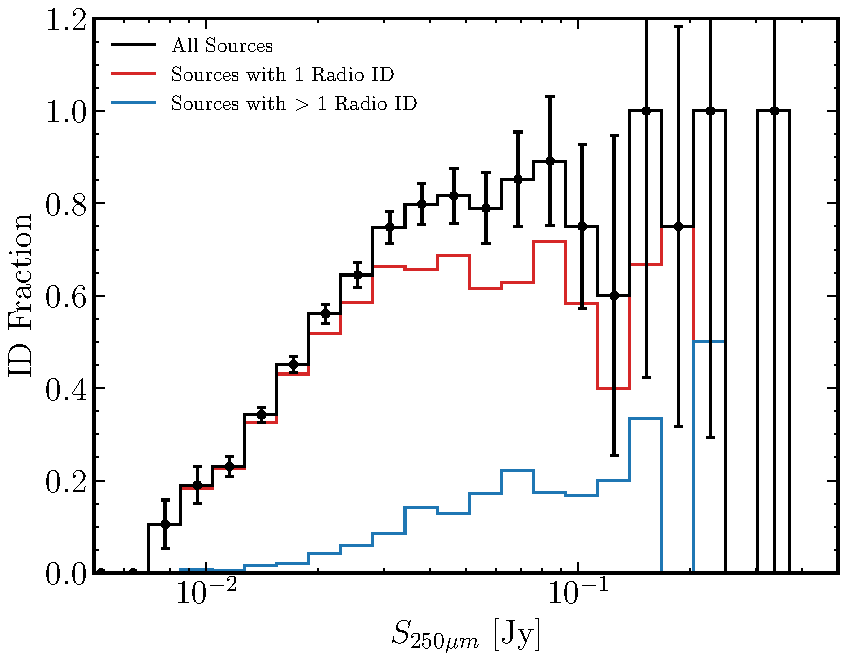
\includegraphics[width=0.8\columnwidth]{Figures/id_fraction_radio.pdf}
	\caption[Identification rate of radio counterparts to \textit{Herschel} sources]{The identification rate of radio counterparts to \textit{Herschel} sources as a function of $250\,\mu$m flux density. The black line shows the identification rate for all \textit{Herschel} positions, while the red and blue lines represent the fraction of those sources that have one or multiple radio counterparts with $P < 0.05$, respectively.}
	\label{fig:id_rate}
\end{figure}

Given that $P_i$ represents the probability of observing a radio counterpart, $i$, with a given radio flux and offset from the far-IR/sub-mm emission by chance, the number of false IDs in a $P$-limited sample is given by

\begin{equation}
    N_{\textrm{False}} = \sum_{P_i < 0.05} P_i,
    \label{eq:false_radio_ids}
\end{equation}

\noindent which is analogous to Equation \ref{eq:false_ids} when using the LR method. From this we estimate that the false identification rate is approximately $0.5\%$ ($N_\textrm{False} \approx 7$). Compared to the fraction of false reliable counterparts identified in the near-IR as part of the H-ATLAS SGP ($\sim 4.8\%$) in Chapter \ref{chapter:Data_Release_3}, the cleanness of the radio sample appears to be much higher. One of the driving factors of this difference is the surface density of radio galaxies compared to near-IR galaxies. The average number of potential counterparts per source for the VIKING analysis was $\sim 5.2$ ($1,005,359$ counterparts to $193,527$ sources), which if we scale to a search radius of $10\,$arcsec reduces to $\sim 2.1$ assuming they are uniformly scattered across the survey. By comparison, there are approximately 1.5 radio sources per \textit{Herschel} source in COSMOS ($10,826$ counterparts to $7,230$ sources).

While the above estimate of the false ID rate was computed for those counterparts with the lowest value of $P$ per source (the \textit{primary} sample), we also observe secondary and tertiary associations that also have $P < 0.05$. For the $1,053$ \textit{Herschel} sources that have secure identifications, $879$ ($83.5\%$) have just a single association, $160$ ($15.2\%$) have two and $14$ ($1.3\%$) have three. The straightforward interpretation of single counterparts is that the radio source is the sole location of the far-IR/sub-mm emission. This would be further supported if the counterpart were particularly luminous and close to the \textit{Herschel} position. The nature of multiple systems, however, is less obvious and is explored in Section \ref{sec:multiple_systems}.

\subsection{Determining SPIRE Positional Errors}

The excellent astrometry of the radio galaxies (with an angular resolution of $0.75\,$arcsec) means that the distribution of the radial separation between the \textit{Herschel} position and the counterpart is almost certainly dominated by the positional errors of the SPIRE detections. We can therefore use this distribution as an independent measure of the typical positional error. During the Likelihood Ratio analysis of the SGP field of \textit{Herschel}-ATLAS, we made the common assumption that the SPIRE positional errors can be modelled with a radially symmetric Gaussian with a width $\sigma_\textrm{pos}$. We then used the \textit{blanks} counting method of \citealt{Fleuren_2012} to estimate that the typical positional error is $\sigma_\textrm{pos} = 2.388\pm0.065\,$arcsec. Here we validate whether this is an appropriate assumption.

Figure \ref{fig:source_counterpart_offset} shows the distribution of offsets between the \textit{Herschel} position and the radio identification. The solid histogram shows the distribution for all primary counterparts, the dotted histogram represents all associations with $P < 0.05$, including secondary and tertiary counterparts, and the dashed histogram shows a single offset for each \textit{Herschel} source where we have taken the average of the radio positions. Assuming random Gaussian errors in R.A. and declination, the distribution of radial offsets should resemble a Rayleigh distribution of the form $R(r, \sigma) \propto \frac{r}{\sigma^2}e^{-\frac{r^2}{2\sigma^2}}$. This results from the fact that for two independent Gaussian random variables with mean zero and standard deviation $\sigma$, as we might expect for the offsets in R.A. and declination ($\Delta\alpha$, $\Delta\delta$), then the offset defined as $r = \sqrt{\Delta\alpha^2 + \Delta\delta^2}$ has a Rayleigh distribution with parameter $\sigma$. The distribution of primary radio identifications is well described by a Rayleigh distribution with a width $\sigma = 1.66\,$arcsec (red line). This is substantially lower than our estimate of the $1\sigma$ positional error measured in Chapter \ref{chapter:Data_Release_3}. The corresponding Rayleigh distribution with $\sigma = 2.388$, for the same number of counterparts, is illustrated with the green line in Figure \ref{fig:source_counterpart_offset}. This represents the distribution of separations we might expect the \textit{Herschel}-VLA associations to take if the probability distribution function for SPIRE positional errors, $f(r)$, took the same form as Chapter \ref{chapter:Data_Release_3}. The narrower distribution implies that the true SPIRE positional errors are smaller than previously estimated.

\begin{figure}
	\centering
	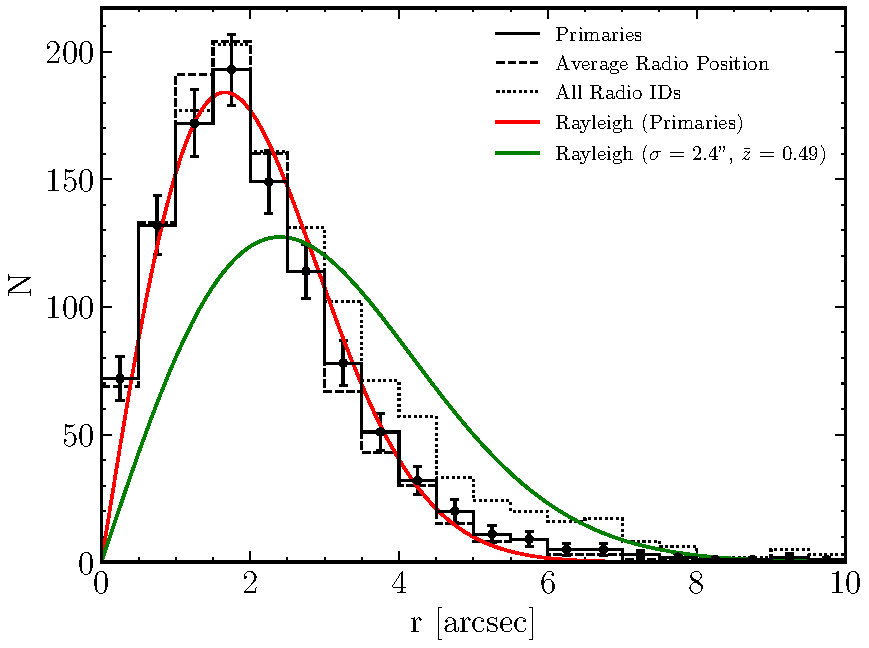
\includegraphics[width=0.8\columnwidth]{Figures/source_counterpart_offsets.pdf}
	\caption[Distribution of radial offsets between \textit{Herschel} sources and radio IDs]{The distribution of separations from the \textit{Herschel} position for the radio sources with $P < 0.05$. The solid black histogram shows the distribution for the primary radio counterparts (those with the lowest $P$ value per \textit{Herschel} source), the dotted black histogram represents all radio IDs (including secondary and tertiary counterparts), and the dashed black histogram represents the radial offset between each \textit{Herschel} source and the average radio position. The latter provides a better description of the positional offsets for multicomponent sources. The red line shows a Rayleigh distribution, $R \propto r/\sigma^2 e^{-r^2/2\sigma^2}$, fitted to the primary counterparts. As detailed in the text, the value of $\sigma$ from the Rayleigh distribution ($\sigma = 1.66\,$arcsec) is an independent estimate of the \textit{Herschel}/SPIRE $250\,\mu$m positional error. We compare this to a Rayleigh distribution with a standard deviation equal to $2.4\,$arcsec, as found in Chapter \ref{chapter:Data_Release_3}. {\color{red}Put into bins of $\sigma$?}}
	\label{fig:source_counterpart_offset}
\end{figure}

\subsection{The Nature of Multiple Identifications}
\label{sec:multiple_systems}

For roughly one sixth of \textit{Herschel} sources in COSMOS, the correct identification is not obvious due to secondary and sometimes tertiary candidates with a low probability of occurring by chance. There are several interpretations for such multiple associations, these include gravitationally lensed images of the \textit{Herschel} galaxy, clustering of true associations, or  unrelated counterparts that have been flux boosted in the far-IR/sub-mm by confusion noise. Studies using interferometric observations at millimeter wavelengths have already shown that $\gtrsim 20\%$ of far-IR/sub-mm sources correspond to multiple galaxies that have been blended in single-dish observations (e.g. \citealt{Karim_2013, Simpson_2015, Stach_2018}). We attempt to understand the cause of our multiple systems by considering whether all the radio associations are related to the dust emission, or faint galaxies blended together in the \textit{Herschel} beam, and if they are related to the far-IR/sub-mm emission, whether they are physically associated with each other.

In Figure \ref{fig:multiples_flux_contribution} we plot the fractional contribution of the brightest radio ID to the total $3\,$GHz flux density of all components, as a function of the $250\,\mu$m flux density. We also show the median contribution from second and third brightest components as red and blue lines, respectively. In a few cases the radio flux is dominated by a single counterpart ($\gtrsim 90\%$). In these cases we may presume that the radio galaxy is the true location of the dust emission, and minor contributions from secondaries are likely to be faint sources along the same line of sight that can otherwise be ignored. However, the majority of our brightest counterparts contribute between $50$ and $70\%$ of the integrated radio flux density, with significant contributions coming from secondaries and tertiaries. The interpretation here is that the dust emission emanates from more than one galaxy that have been blended together by the SPIRE beam. {\color{red}Make it clear here that the dust emission does not need to come from BOTH galaxies.}

\begin{figure}
	\centering
	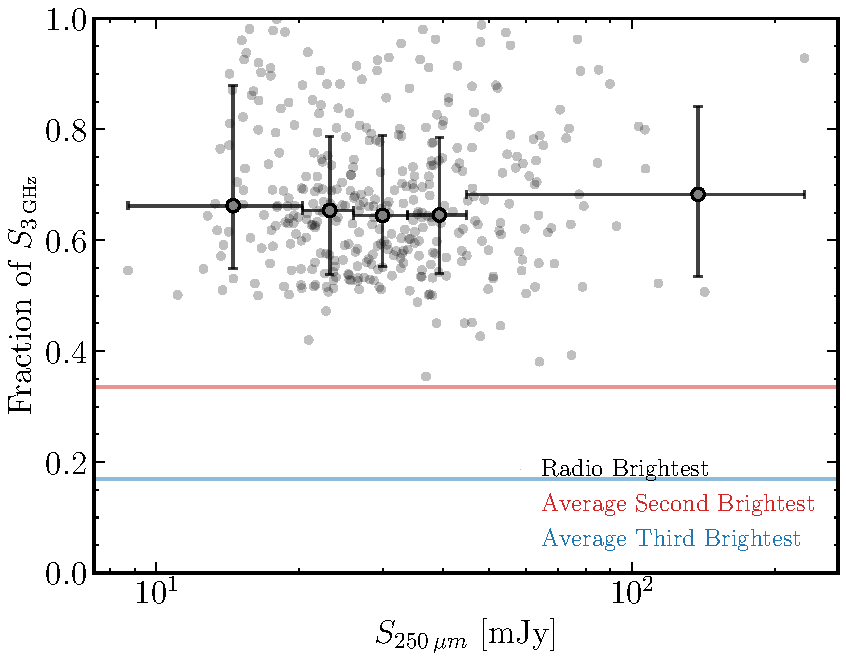
\includegraphics[width=0.8\columnwidth]{Figures/multiples_flux_contribution.pdf}
	\caption[Contribution to total radio flux from multicomponent radio sources]{The fraction of the integrated $3\,$GHz flux contributed by the brightest radio counterpart, as a function of the $250\,\mu$m flux of multicomponent \textit{Herschel} sources. The median contribution by the second and third brightest components are shown with red and blue lines, respectively, while the median contribution from the brightest radio sources is illustrated by a series of error bars. The vertical errors correspond to the $16$th to $84$th percentiles. {\color{red}Make prettier - remove lines.}}
	\label{fig:multiples_flux_contribution}
\end{figure}

Having established that the majority of our \textit{Herschel} sources with multiple secure radio IDs are likely to be formed from multiple, confused galaxies, we now question whether these might be physically associated systems. In Figure \ref{fig:multiples_separation} we plot the radial separation between two secure IDs as a function of the difference in their photometric redshift. The photometric redshifts were obtained from the COSMOS2020 catalogue using the \texttt{LePhare} spectral template fitting code (\citealt{Arnouts_1999, Ilbert_2006}) applied on the observed photometry. The high fraction of sources that have secure radio IDs with redshifts within $0.1$ of each other implies a significant fraction of the sources that resolve into multiple distinct galaxies are indeed physically associated with each other. At the median redshift of our VLA sources, $z_\textrm{median} = 0.91$, the angular separation between IDs corresponds to physical distances between $\sim 10$ and $100\,$kpc. The prevailing theory for DSFG formation is that they are the result of major mergers (\citealt{Ivison_2002, Smail_2004, Ivison_2007, Engel_2010, Hayward_2011}) that induce a starbursting phase and boost the far-IR/sub-mm flux. The lack of very small offsets ($\lesssim 2\,$arcsec) suggests that these components are not likely to be lensed images, but could be interacting galaxies and mergers, and given the large range of separations, may further indicate the presence of clusters of galaxies.

\begin{figure}
	\centering
	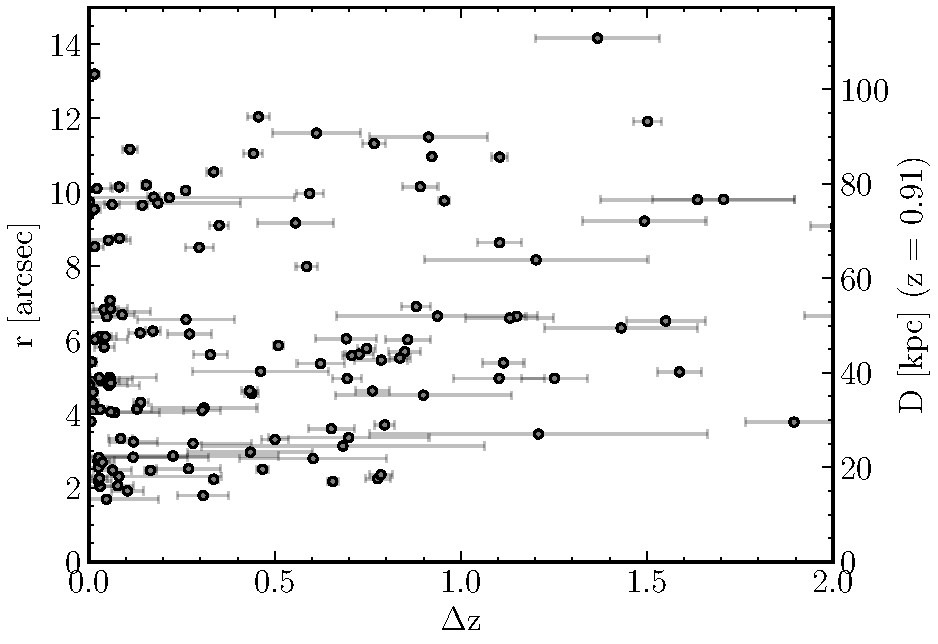
\includegraphics[width=0.8\columnwidth]{Figures/multiples_separation.pdf}
	\caption[Physical separation between radio IDs for a single \textit{Herschel} source]{\textit{Herschel} sources with multiple $P < 0.05$ radio counterparts in the plane of $\Delta z$ and $r$, representing the difference in the photometric redshift of the radio sources and the separation from each other. This figure illustrates that those \textit{Herschel} sources with multiple associations have radio separations between $\sim 10$ and $100\,$kpc (at an average redshift of $z = 0.91$) and are often observed at the same redshift. {\color{red}May want to change having secondary "physical" scale.}}
	\label{fig:multiples_separation}
\end{figure}

\subsection{Missing Identifications}

For $271$ \textit{Herschel} sources ($> 30\,$mJy) we do not observe any radio counterpart within $10\,$arcsec of the \textit{Herschel} position, or we observe a potential counterpart, but it is not considered a secure identification ($P < 0.05$). This corresponds to approximately $20\%$ of the total sample. If we allow the counterparts to be considered secure to $P < 0.1$, then the number of blanks reduces by only $17$ sources to $254$ (note that the maximum $P$ value in this study is only $\sim 0.1$). This tells us that the majority of our blank fields are not due to a large number of tentative crossmatches, but the result of a large number of \textit{Herschel} positions where no possible radio counterparts are observable.

There are several reasons why we might not observe true counterparts. The most obvious reason is that a small number of \textit{Herschel} detections are likely to be spurious, though we remove most of this problem by considering sources with $S_{250} > 30\,$mJy. Secondly, the true counterpart could lie outside of the search radius. However, if the $1\sigma$ positional errors are of order $1.66\,$arcsec, then a search radius of $10\,$arcsec corresponds to $\sim 6\sigma$. The probability of the true counterpart being present outside this radius is vanishingly small. A third possibility is that the \textit{Herschel} galaxy lies at a high redshift ($z > 3$), beyond the depth of our $3\,$GHz observations (\citealt{Eales_2003}). We can test this by comparing the radio-detected and radio-undetected \textit{Herschel} populations. In Figure \ref{fig:blank_fir_colours} we show the $S_{500}/S_{350}$ against $S_{250}/S_{350}$ colour-colour diagram for our blank fields compared to our \textit{Herschel}-VLA matches. For illustration purposes, we show the path taken by a galaxy with a dust temperature of $30\,$K and dust emissivity index, $\beta = 2$, from $z = 0$ to $z = 4$ (right to left). There is no clear difference between the two populations, meaning that the blanks are not necessarily at higher redshifts.

\begin{figure}
	\centering
	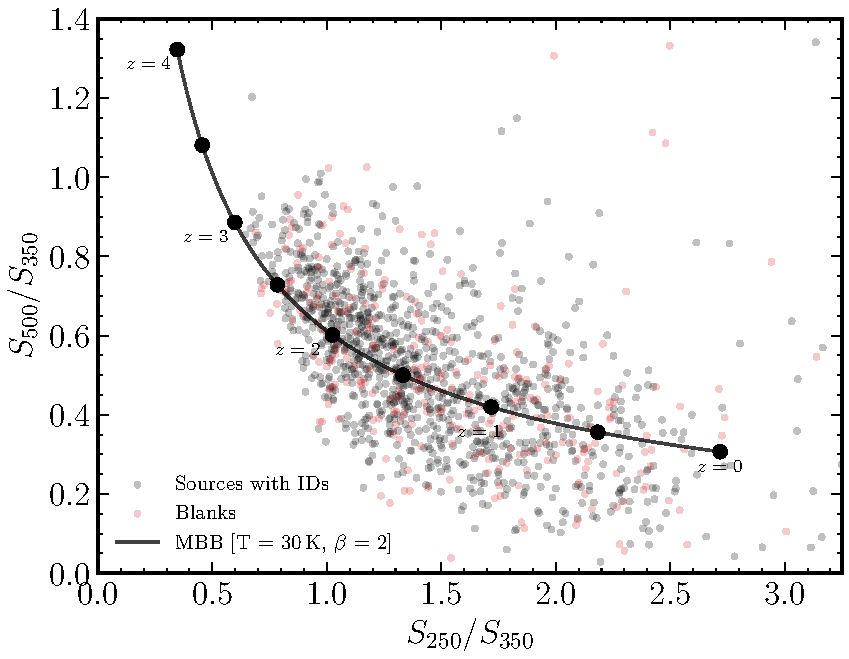
\includegraphics[width=0.8\columnwidth]{Figures/blank_fir_colours.pdf}
	\caption[$S_{500}/S_{350}$ against $S_{250}/S_{350}$ plot of sources with and without radio IDs]{Colour-colour diagram ($S_{500}/S_{350}$ against $S_{250}/S_{350}$) of \textit{Herschel} sources with radio IDs (black points) and for those in which we do not observe any possible radio counterpart or the counterparts we do observe have $P > 0.05$ (red points). The solid black line represents the path taken by a galaxy with a single dust temperature of $30\,$K and dust emissivity spectral index, $\beta = 2$, from $z = 0$ to $z = 4$.}
	\label{fig:blank_fir_colours}
\end{figure}

The final hypothesis that we can provide for our blank fields is that they represent sources that have been resolved into multiple galaxies with flux densities too faint to be detected in the VLA observations. Given the fraction of multiple IDs we observe and the expectation from previous studies that at least 20\% of far-IR/sub-mm sources correspond to multiple galaxies, we believe it is not an unreasonable justification for these sources.

\section{\textit{Herschel} Galaxies in Relation to the Star-Formation Main Sequence}

The evolutionary stage of our \textit{Herschel} selected galaxies can be inferred from their location with respect to the star-formation main sequence; the tight correlation between star formation rate and stellar mass, $M_*$, for star-forming galaxies (see Section \ref{sec:star_forming_main_sequence}). The tight correlation observed both in the local Universe and at high redshifts suggests a long-lasting mode of star formation in galaxies with steady star formation histories. This relationship evolves to higher SFRs with increasing redshift such that SFRs of main sequence galaxies at a given stellar mass are roughly ten times larger at $z\sim1$ than they are today (\citealt{Noeske_2007}). Outliers are observed above and below the main sequence, typically referred to as starbursts that have elevated SFRs likely due to gas-rich major mergers or dense nuclear star formation regions (\citealt{Daddi_2010}), and passive galaxies with quenched star formation and a reduction in cold gas that has caused it to fall off the main sequence.

Recent works have studied \textit{Herschel}-detected DSFGs in relation to the main sequence, with some studies finding that they lie above the main sequence (e.g. \citealt{Hainline_2011}), while others suggesting that their high SFRs are proportional to their mass, locating them at the high-mass, high-SFR end of the main sequence (e.g. \citealt{Michalowski_2012a}). Naturally, \textit{Herschel}-detected galaxies are selected based on their continuum dust emission, and as such our sample will be SFR-limited towards large dust masses and thus high SFRs. The stellar masses of our \textit{Herschel} galaxies are taken to be the stellar masses of our primary radio IDs, estimated from the template fitting of \texttt{LePhare} mentioned earlier. We measure the star formation rates of our galaxies by first calculating their IR luminosity ($8 - 1,000\,\mu$m) from fitting a one temperature component SED to the \textit{Herschel} photometry, and then using the $\textrm{L}_{\textrm{IR}}$ calibration for SFR given by \citealt{Murphy_2011}:

\begin{equation}
	\textrm{SFR}_{\textrm{IR}} [M_\odot\textrm{yr}^{-1}] = 3.88\times10^{-44}\textrm{L}_{\textrm{IR}} [\textrm{erg s}^{-1}].
	\label{eq:LIR_SFR_calibration}
\end{equation}

For comparison purposes, we assume the star-formation main sequence takes the form given in \citealt{Scoville_2017}. This assumes that the shape of the main sequence with stellar mass follows 

\begin{equation}
	\textrm{SFR}_{\textrm{MS}} = 10^{[1.72-\textrm{log}(1+10^{\textrm{log}M_*-10.31})^{-1.07}]},
	\label{eq:scoville_ms}
\end{equation}

\noindent and that it evolves with redshift according to $(1+z)^{2.9}$. Early forms of the MS assumed single power laws of the form SFR $\propto M_*^N$ with values of $N$ typically around one (e.g. \citealt{Daddi_2007, Elbaz_2007}). More recent consensus is that the MS is roughly linear up to a critical mass where it flattens toward higher masses. The simplest explanation for this flattening would be if the growth of galaxies along the MS does not result in a proportional increase in the cold gas reservoir, or if the star formation efficiency decreases. The form of the MS by \citealt{Scoville_2017} that is used here defines a plateauing in the MS above a critical mass $\sim 10^{10.5}\,M_\odot$, as can be seen in Figure \ref{fig:star_formation_ms}. The conclusions we draw from the location of our \textit{Herschel} galaxies in relation to the MS will be substantially affected by the deviation from a linear power law, but this choice is backed by many studies that have reported evidence that the MS flattens at high masses (e.g. \citealt{Magnelli_2014, Whitaker_2014, Schreiber_2015, Tomczak_2016}).

\begin{figure}
	\centering
	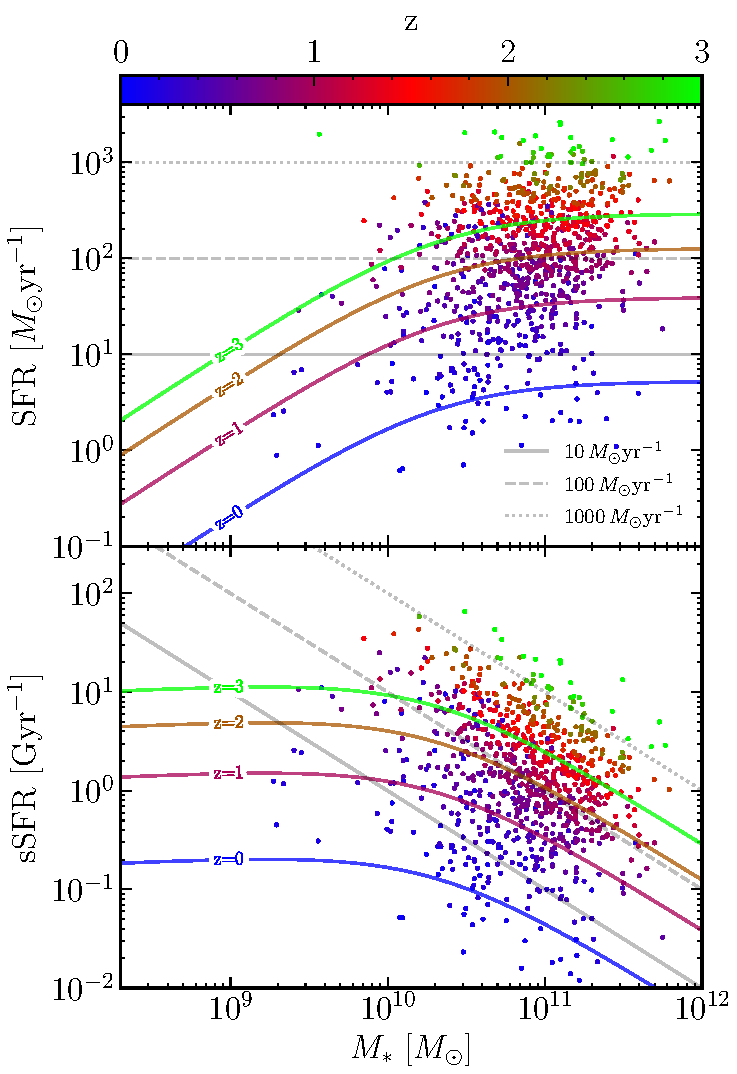
\includegraphics[width=0.8\columnwidth]{Figures/star_formation_ms.pdf}
	\caption[The $M_*$-SFR and $M_*$-sSFR planes of \textit{Herschel} galaxies between $0 < z < 3$]{The stellar mass - star formation rate (top) and the stellar mass - specific star formation rate (bottom) relations at $0 < z < 3$. In both panels the sample of \textit{Herschel} galaxies is coloured according to their photometric redshift from COSMOS2020. The solid, dashed and dotted lines mark the loci of constant star formation rates of $10$, $100$ and $1,000\,M_\odot$yr$^{-1}$, respectively. The coloured lines indicate the main sequence of star forming galaxies defined by \citealt{Scoville_2017} at $z = 0, 1, 2$ and $3$.}
	\label{fig:star_formation_ms}
\end{figure}

The top panel of Figure \ref{fig:star_formation_ms} shows that at the redshift of each galaxy, the \textit{Herschel} galaxies are significantly above the MS in most cases. This result is not necessarily surprising given the SFR limits imposed by large-area \textit{Herschel} surveys. For the highest redshifts ($z \gtrsim 2.5$) we measure star formation rates in excess of $1,000\,M_\odot$yr$^{-1}$. These sources have IR luminosities $> 10^{12.8}\,L_\odot$, which puts them in the same category as the most massive Ultraluminous Infrared Galaxies (ULIRGs) and Hyperluminous Infrared Galaxies (HyLIRGs). We find it constructive to express this figure in terms of the specific star formation rate, sSFR, which provides a fairer comparison among galaxies of different sizes (lower panel of Figure \ref{fig:star_formation_ms}). The sSFR of our sample informs us about how efficiently the galaxies are forming their stellar mass, relative to their existing stellar content. The sSFR of a galaxy is a useful indicator of the current star formation compared to past star formation since, at a constant rate of <SFR>, the stellar mass is proportional to <SFR> $\times t_{\textrm{age}}$ where $t_{\textrm{age}}$ is the age of the galaxy, ignoring the effects of recycling. This means that if we assume a constant star formation rate, the sSFR of a galaxy scales as the inverse of the age of the galaxy. The bottom panel shows that the higher mass galaxies have typically lower specific SFRs than less massive ones. There is previous evidence to suggest that the major contribution to star formation in a galaxy starts later for less massive galaxies, which would manifest itself as a higher sSFR. This implies that massive galaxies formed their stars earlier whereas less massive galaxies are still actively star forming, hence their elevated sSFR (e.g. \citealt{Brinchmann_2000, Juneau_2005, Bell_2005, Caputi_2006, Reddy_2006, Noeske_2007}). At first sight our sample would be in agreement with this "cosmic downsizing", however, we add the caveat that our $L_{\textrm{IR}}$ limits at each redshift create an sSFR limit diagonal in the sSFR-$M_*$ plane from low mass, high sSFR to high mass, low sSFR.

There is no universal definition for a starburst galaxy, the term is applied to a diverse range of galaxy populations. However, common to all starbursting populations is that they have SFRs that are much higher than their long-term average. We consider a star-forming galaxy to be defined as in a "starbursting phase", if the length of time it would take to form its observed stellar mass is a small fraction of the age of the Universe at the redshift of the galaxy. In this sense, we are observing these galaxies during an intense period of star formation and as such we are directly observing these galaxies as they form the bulk of their stellar mass. For constant SFR, the total mass of stars in a galaxy would be produced in a doubling timescale given by $\tau = 1/$sSFR, which we standardize by the age of the Universe at the redshift of each galaxy, $t_z$. In Figure \ref{fig:tau_against_age} we show the distribution of $\tau/t_z$ for our \textit{Herschel} galaxies. We see that the average doubling timescale is approximately $10\%$ of the age of the Universe, which would imply short starburst duty cycles. It also illustrates that the fraction of time spent in this phase of evolution is shorter for higher redshift galaxies - which is to say that at higher redshifts, such galaxies are forming the bulk of their stellar mass more quickly.

\begin{figure}
	\centering
	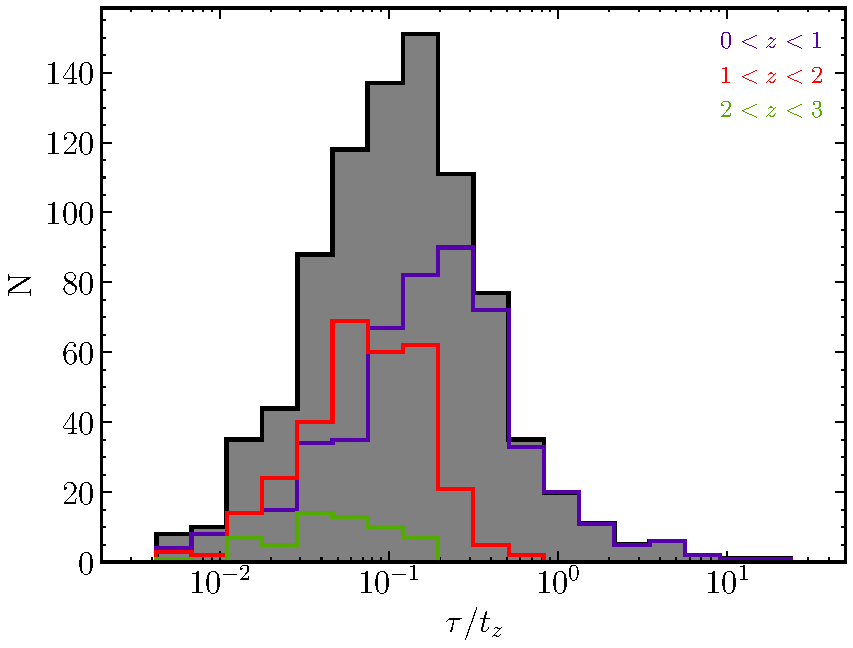
\includegraphics[width=0.8\columnwidth]{Figures/tau_against_age.pdf}
	\caption[Doubling timescale of \textit{Herschel} galaxies]{The distribution of the doubling timescale, $\tau = 1/$sSFR, divided by the age of the Universe at the redshift of the galaxy. The figure shows that the typical time it would take to form the stellar masses of our \textit{Herschel} galaxies is approximately $10\%$ of the age of the Universe at which the galaxy is observed. The purple, red and green lines represent sub-samples at redshift intervals of $0 < z < 1$, $1 < z < 2$ and $2 < z < 3$.}
	\label{fig:tau_against_age}
\end{figure}

The galaxies observed at $z \gtrsim 2$ have exceptional star formation rates that make them ideal candidates for being the progenitors to the massive elliptical galaxies in the local Universe. In this scenario, these galaxies represent a fixed stage in the evolutionary sequence toward a local massive, passively evolving elliptical. Assuming a merger history where gas-rich disk galaxies collide and ignite an intense starbursting phase due to rapid compression and cooling of the gas. This phase of high SFR produces the vast quantities of dust and the young, blue stars that make this evolutionary stage bright in the far-infrared and sub-mm wavelengths. With limited gas supply and high SFRs, this burst is expected to be short-lived ($\sim 10^7 - 10^8\,$yr; \citealt{Greve_2005, Tacconi_2006, Hickox_2012}). Star formation ceases and the galaxy secularly evolves to an elliptical galaxy with an old stellar population. Much of this evolutionary connection is based on similarities in the two populations, notably the distribution of their sizes, stellar masses and internal velocities (\citealt{Toft_2014}). Given our \textit{Herschel} sample are found at the high mass end of the $M_*$-SFR plane, and are rapidly forming their stellar content, we expect they would later evolve to be massive galaxies with stellar populations of similar ages. It therefore seems likely that our sample of \textit{Herschel}-detected galaxies are early Universe versions of elliptical galaxies being observed during a rapid mass-building phase.

\section{Identifying Multiwavelength Counterparts of DSFGs from Blank Fields}

The identification of radio counterparts to \textit{Herschel} sources in COSMOS has shown the efficiency with which we can unambiguously locate at least one very likely optical/infrared association. However, as mentioned earlier, this method is not practical on the scale of the \textit{Herschel} surveys conducted to date, and thousands of \textit{Herschel} sources currently do not have optical/IR identifications due to the uncertainty that come from directly matching to the low resolution dust emission. With our high identification rate ($\sim 80\,\%$) we aim to show proof-of-concept for a future program that would be able to identify the characteristic signatures of DSFGs in a wide area blank field covered by \textit{Herschel}, using the multiwavelength properties of our sample.

In reference to the LR method of Chapter \ref{chapter:Data_Release_3}, we note that statistical analyses like this are dependent on one or two properties; in this case the radial separation from the far-IR/sub-mm source and the flux density in a single band. We propose that a more efficient method would be to train some machine learning algorithm to detect the signs of a DSFG from the set of observables we typically have in a wide field photometric survey. The first hurdle is that an effective machine learning algorithm requires a training set that represents a complete census of the target population. Any sub-sample of the target population that is not represented in the training set will not have any chance of being selected by the algorithm. We already know that we are missing $\sim20\,\%$ of the \textit{Herschel} population in the COSMOS field, which, if they had distinctly different properties from the rest of the sample, would not be recovered when applied to future fields. We have not found evidence to suggest that these objects represent a distinct group of galaxies, and the most obvious explanation for missing IDs, their redshift, does not appear to be the cause. In the following we assume that our sample of $1,053$ \textit{Herschel} sources for which we have photometry from UV to the radio form a representative sample, and use the multiwavelength data to discern whether DSFGs can be cleanly separated from non-DSFGs in the field.

Table \ref{tab:smg_coverage} shows the UV-IR coverage provided by COSMOS2020, including the fraction of our DSFGs that have observations in each waveband, which in most cases is between $70$ and $85\%$. In Figure \ref{fig:smg_colours} we plot a range of colour-colour plots that, from top to bottom, progressively samples the UV to IR bands. Given the wide redshift range of our galaxies it is unlikely that we would find any single feature that would help distinguish most of our \textit{Herschel} galaxies from the background galaxies (grey histograms). However, Figure \ref{fig:smg_colours} does show the possible separation between DSFGs and non-DSFGs that can be made at a given redshift, with the DSFGs almost always having redder colours. This is not particularly surprising given the dust reddening that we would expect; previous studies have already illustrated that they are generally more red in optical to near-IR colours (e.g. \citealt{Smail_2002, Dannerbauer_2004, Wang_2012, Chen_2016}), resulting in optical colour cuts previously being used to identify possible counterparts (e.g. \citealt{Michalowski_2012b}).

\begin{table}
    \centering
    \begin{tabular}{p{4cm}|p{1.5cm}|p{2cm}|p{2cm}|p{1.5cm}|p{1.5cm}}
        \hline
		\hline
		Instrument / Telescope & Band & Wavelength [$\mu$m] & Band Width [$\mu$m] & $N_{\textrm{DSFG}}$ & Percent \\
		\hline
		\hline
		GALEX & FUV & 0.1526 & 0.0224 & 283 & 26.90 \\
		& NUV & 0.2307 & 0.0791 & 475 & 45.15 \\
		\hline
		MegaCam / CFHT & $u$ & 0.3709 & 0.0518 & 847 & 80.51 \\
		\hline
		Suprime-Cam / & $IB427$ & 0.4266 & 0.0207 & 805 & 76.52 \\
		Subaru & $B$ & 0.4488 & 0.0892 & 909 & 86.41 \\
		& $IB464$ & 0.4635 & 0.0218 & 792 & 75.29 \\
		& $g^+$ & 0.4804 & 0.1265 & 874 & 83.08 \\
		& $IA484$ & 0.4851 & 0.0229 & 844 & 80.23 \\
		& $IB505$ & 0.5064 & 0.0231 & 837 & 79.56 \\
		& $IA527$ & 0.5261 & 0.0243 & 835 & 79.37 \\
		& $V$ & 0.5487 & 0.0954 & 904 & 85.93 \\
		& $IB574$ & 0.5766 & 0.0273 & 837 & 79.56 \\
		& $IA624$ & 0.6232 & 0.0300 & 861 & 81.84 \\
		& $r^+$ & 0.6305 & 0.1376 & 915 & 86.98 \\
		& $IA679$ & 0.6780 & 0.0336 & 849 & 80.70 \\
		& $IB709$ & 0.7073 & 0.0316 & 852 & 80.99 \\
		& $NB711$ & 0.7121 & 0.0072 & 845 & 80.32 \\
		& $IA738$ & 0.7361 & 0.0324 & 857 & 81.46 \\
		& $i^+$ & 0.7693 & 0.1497 & 876 & 83.27 \\
		& $IA767$ & 0.7694 & 0.0243 & 848 & 80.61 \\
		& $NB816$ & 0.8150 & 0.0120 & 903 & 85.84 \\
		& $IB827$ & 0.8243 & 0.0343 & 855 & 81.27 \\
		& $z^+$ & 0.8978 & 0.0365 & 913 & 86.79 \\
		& $z^{++}$ & 0.9063 & 0.1335 & 883 & 83.94 \\
        \hline
		Hyper Suprime-Cam / & $g$ & 0.4847 & 0.1383 & 919 & 87.36 \\
		Subaru & $r$ & 0.6219 & 0.1547 & 920 & 87.45 \\
		& $i$ & 0.7699 & 0.1471 & 922 & 87.64 \\
		& $z$ & 0.8894 & 0.0766 & 922 & 87.64 \\
		& $y$ & 0.9761 & 0.0786 & 922 & 87.64 \\
		\hline
		ACS / HST & F814W & 0.8333 & 0.2511 & 613 & 58.27 \\
		\hline
		VIRCAM / & $Y$ & 1.0216 & 0.0923 & 738 & 70.15 \\
		VISTA & $NB118$ & 1.1909 & 0.0112 & 442 & 42.02 \\
		& $J$ & 1.2525 & 0.1718 & 735 & 69.87 \\
		& $H$ & 1.6466 & 0.2905 & 740 & 70.34 \\
		& $K_s$ & 2.1557 & 0.3074 & 740 & 70.34 \\
		\hline
		IRAC / & ch1 & 3.5686 & 0.7443 & 884 & 84.03 \\
		Spitzer & ch2 & 4.5067 & 1.0119 & 883 & 83.94 \\
		& ch3 & 5.7788 & 1.4082 & 881 & 83.75 \\
		& ch4 & 7.9958 & 2.8796 & 876 & 83.27 \\
		\hline
		\hline
    \end{tabular}
    \caption[UV to IR coverage of our \textit{Herschel} galaxies from COSMOS2020]{The UV to IR data in the COSMOS2020 catalogue. The final two columns show the number of \textit{Herschel} sources with an observation in the given photometric band and the fraction of these sources as a percentage.}
    \label{tab:smg_coverage}
\end{table}

\begin{figure}
	\centering
	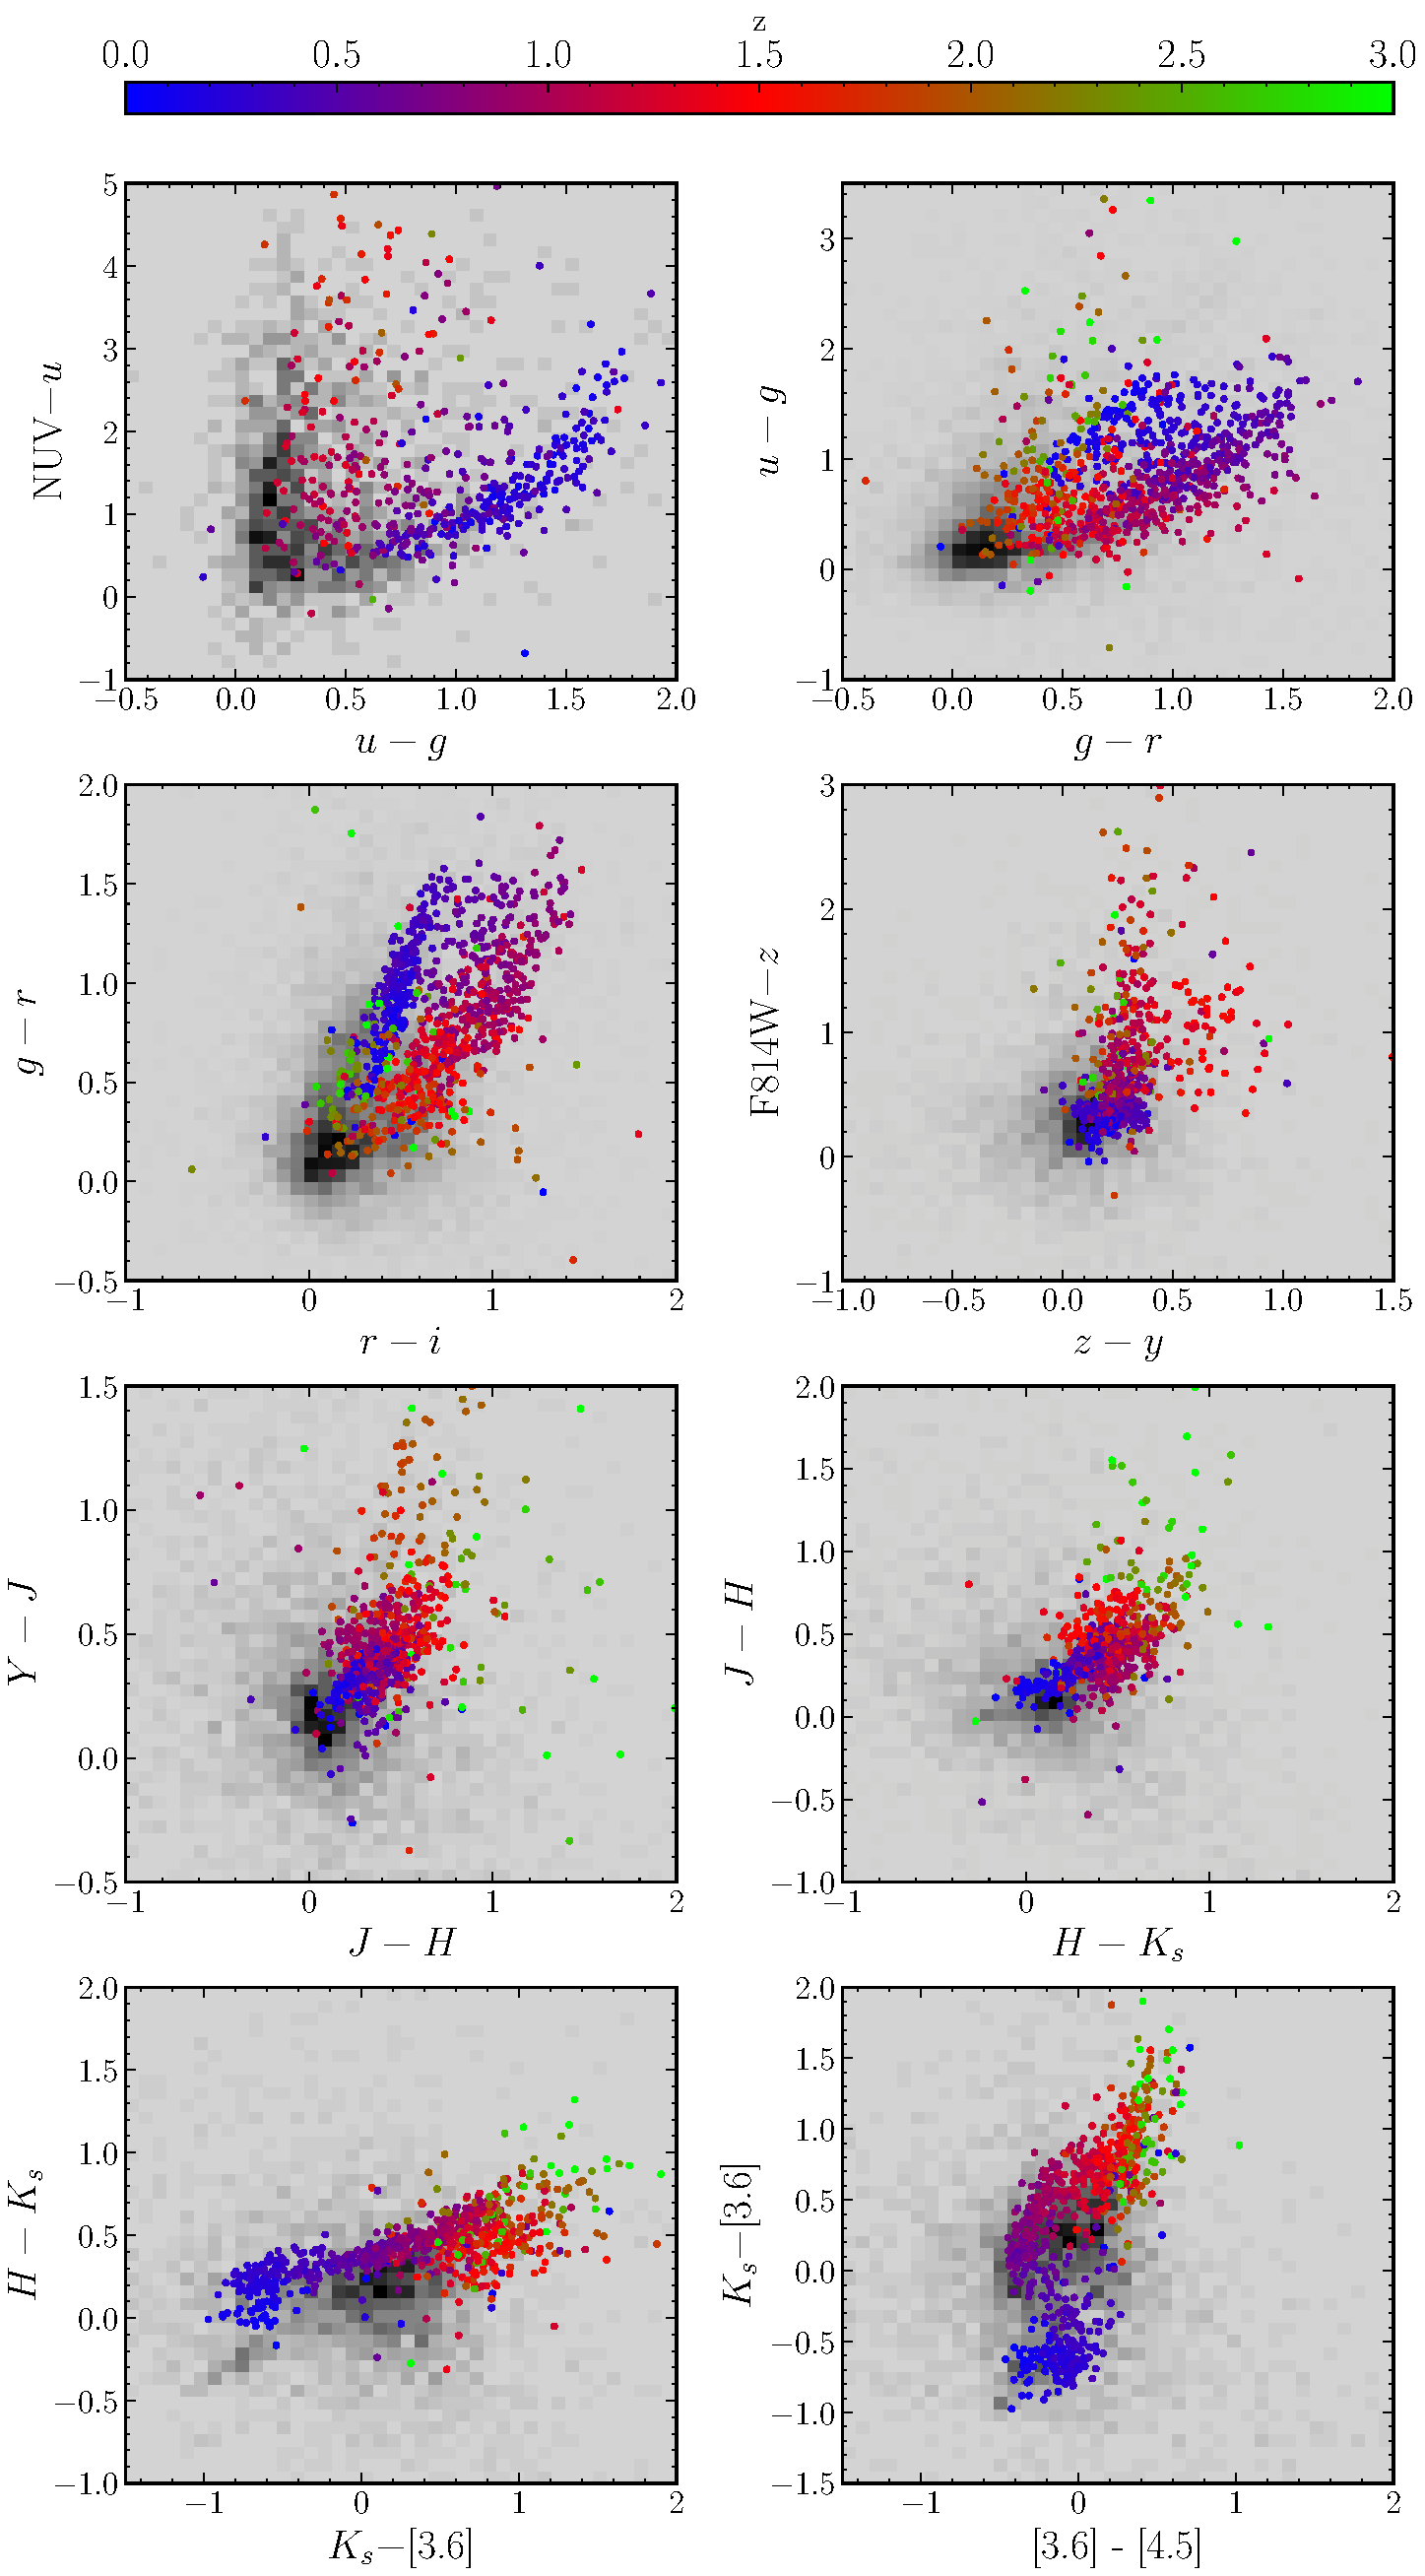
\includegraphics[width=0.85\columnwidth, height=0.9\textheight]{Figures/smg_colours.pdf}
	\caption[Selection of colour-colour diagrams]{A selection of colour-colour spaces for the multiwavelength counterparts to our \textit{Herschel} sources, coloured by their photometric redshift. The 2D histograms (black) show the distribution of the full COSMOS2020 catalogue. The colour-colour plots are selected to explore the full UV to IR spectrum, from the top row to the bottom.}
	\label{fig:smg_colours}
\end{figure}

We recall in Chapter \ref{chapter:Data_Release_3} that we were able to reliably match $\sim 57\%$ of \textit{Herschel} sources in the South Galactic Pole field of H-ATLAS with a near-infrared counterpart. This itself depended on the fraction of true counterparts that could be observed on the VIKING images, $Q$, which was $\sim 84\%$. We propose that had we a priori knowledge about a selection of the optical/IR colours of DSFGs in comparison to non-DSFGs, we might be able to use this information to improve on our recovery percentage. Moreover, without having to observe both the dust emission and a coincident counterpart means that we would not have to account for the value of $Q$.

To illustrate how useful additional photometric coverage would be in identifying dusty galaxies, we start from the assumption that we have already detected a \textit{Herschel} source and observed nearby optical/IR counterparts. In our simple situation our question is - if there is one counterpart near the \textit{Herschel} source, how confident can we be in our binary classification of DSFG or non-DSFG? Essentially, we shall assume here that the surface density of DSFGs and non-DSFGs are the same, so as not to worry about trying to recreate a typical photometric survey. In Figure \ref{fig:smg_nonsmg} we show the histograms of different observed properties (the angular separation and a selection of colours). As would be expected, the most definitive way of deciphering between the two populations is in the separation between source and counterpart. To illustrate how well each observable could be used individually, we show the DSFG fraction in the bottom panel, defined as $f_\textrm{DSFG} = N_\textrm{DSFG}/(N_\textrm{DSFG}+N_\textrm{non-DSFG})$. We determine this fraction by randomly selecting $100$ sources from our catalogue and $100$ other glaxies from the COSMOS2020 catalogue, and plotting the median fraction for $1,000$ iterations. We then modelled this fraction using a sigmoid function. The most effective observables would be those in which we observe a sharp change in $f_\textrm{DSFG}$ between a very high and very low value. While the radial separation varies from very close to one at small radii to zero at high radii, it is slowly evolving (as background galaxies are observed with a predictable radial dependence, unlike colours where they may have preference for particular ranges). While the colours typically do not reach as high values of $f_\textrm{DSFG}$, telling us that there are no regions of colour space where we only expect to observe DSFGs, which would help immediately classify some fraction of \textit{Herschel} galaxies, we do observe some sharper transitions. This gives credit to the idea that a combination of colours, alongside the separation from the source, could be used to define a plane of separation with reasonably minimized contamination.

\begin{figure}
	\centering
	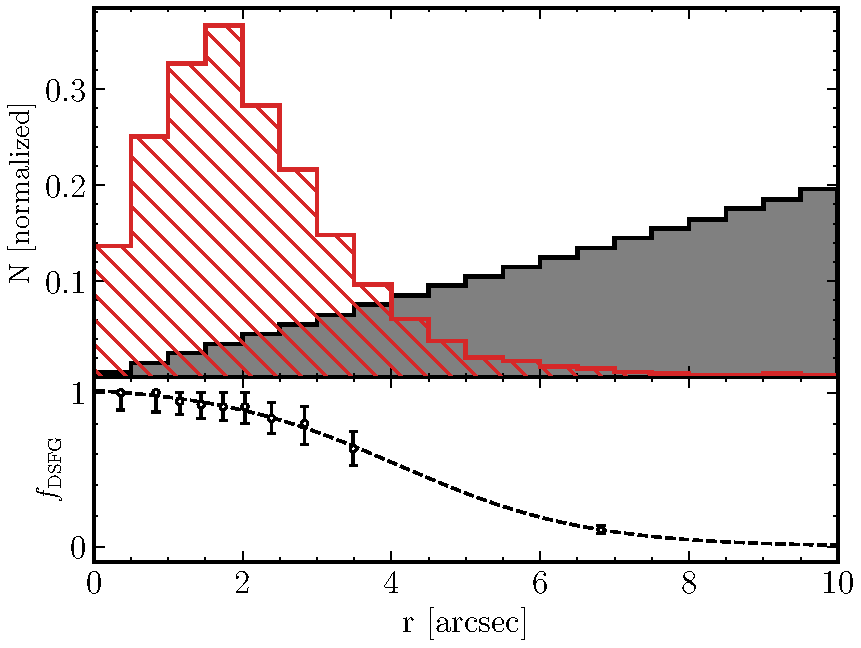
\includegraphics[width=0.49\columnwidth, height=0.25\textheight]{Figures/offset_smg.pdf}
	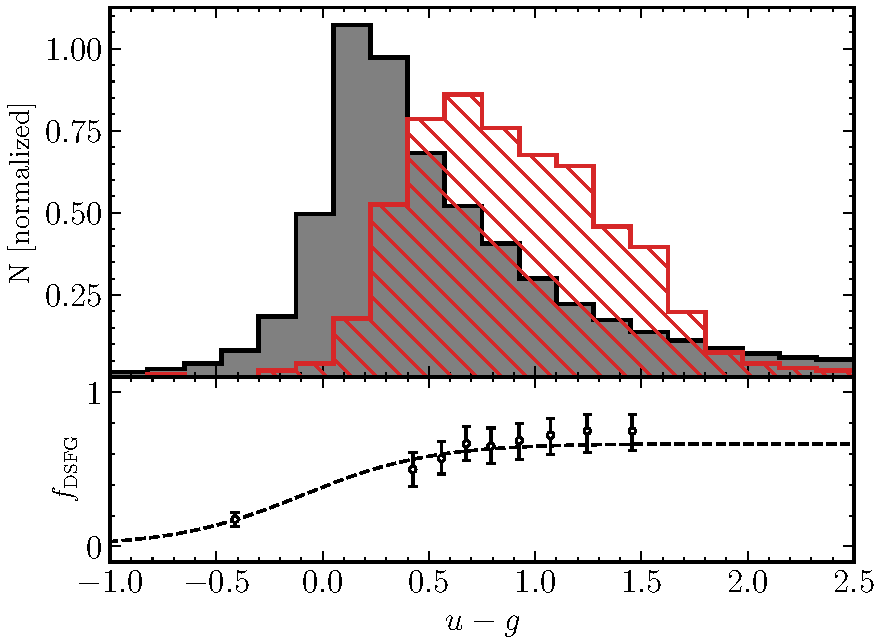
\includegraphics[width=0.49\columnwidth, height=0.25\textheight]{Figures/ug_smg.pdf}
	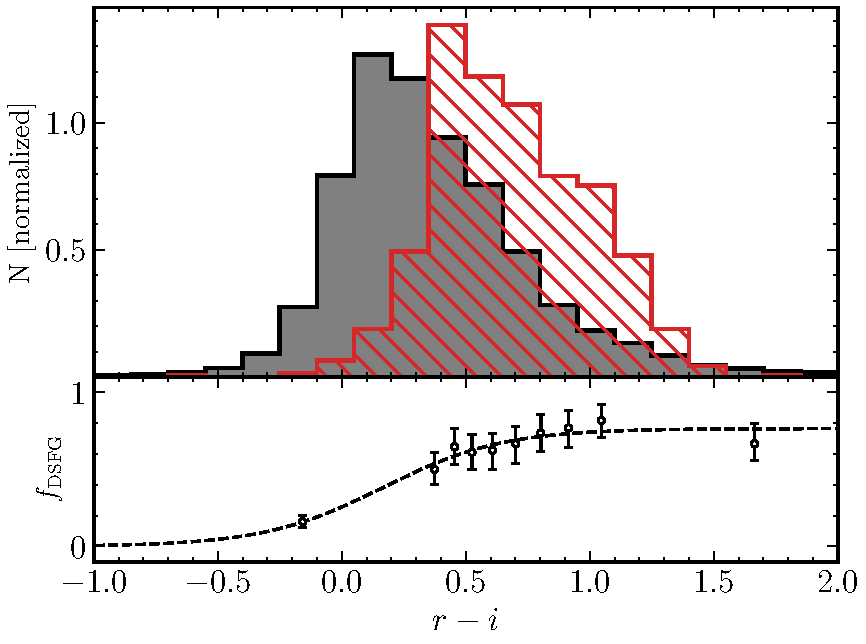
\includegraphics[width=0.49\columnwidth, height=0.25\textheight]{Figures/ri_smg.pdf}
	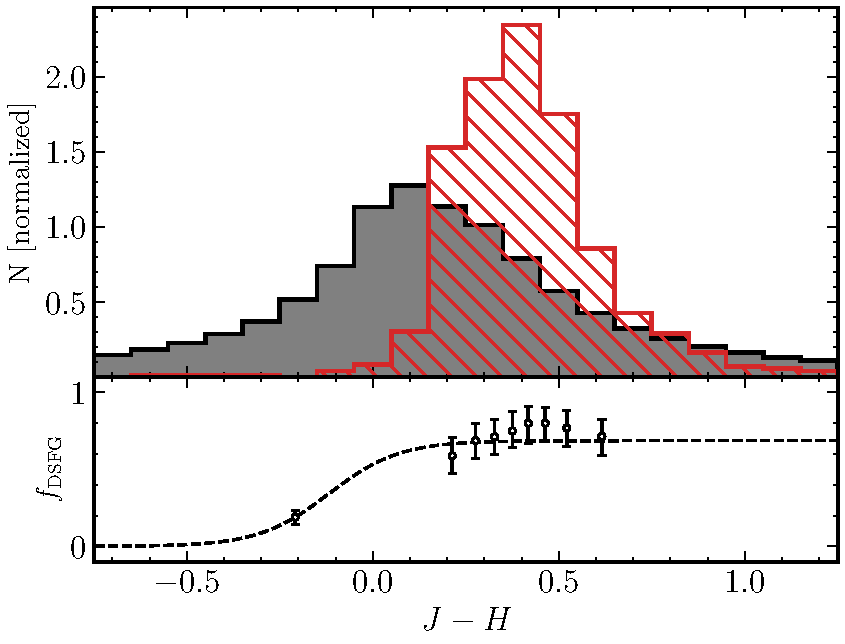
\includegraphics[width=0.49\columnwidth, height=0.25\textheight]{Figures/JH_smg.pdf}
	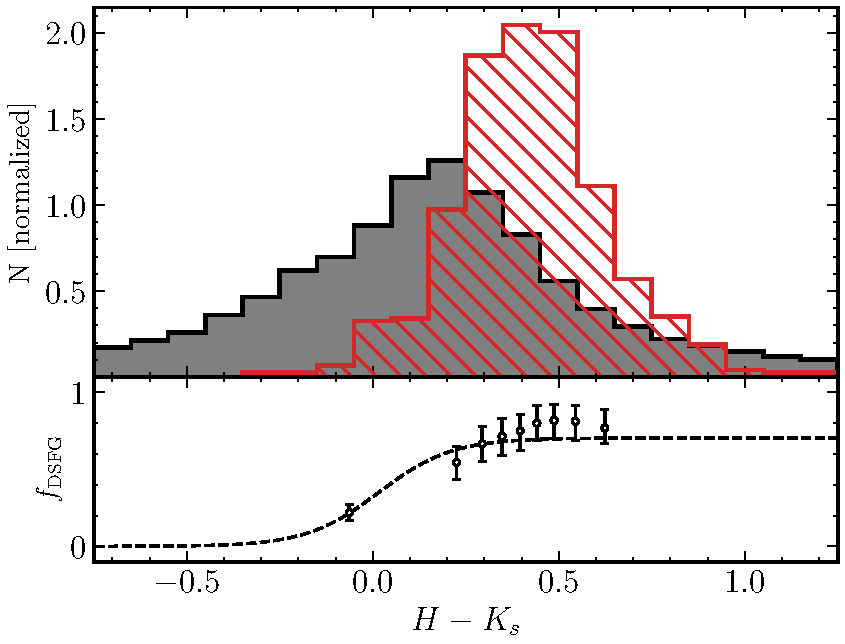
\includegraphics[width=0.49\columnwidth, height=0.25\textheight]{Figures/HK_smg.pdf}
	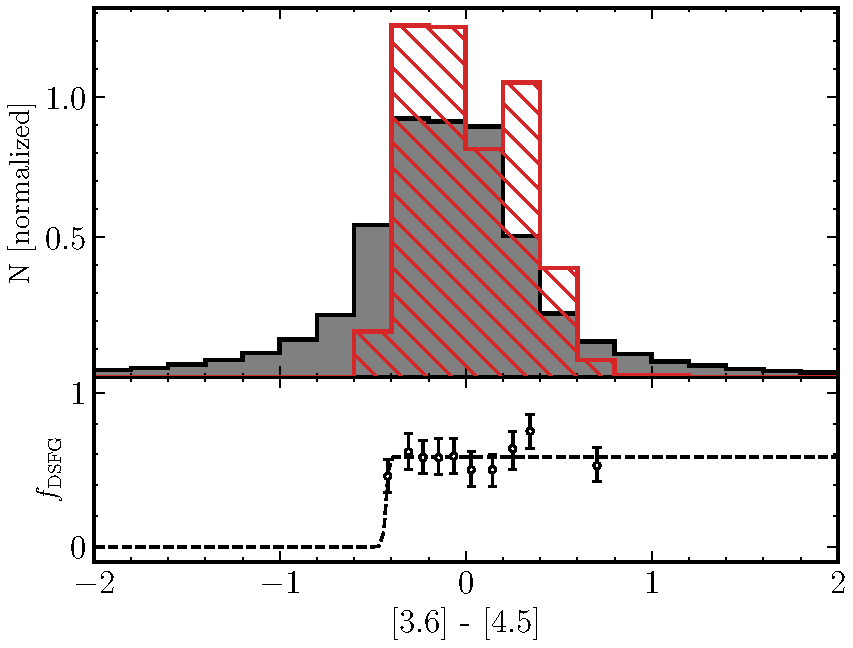
\includegraphics[width=0.49\columnwidth, height=0.25\textheight]{Figures/3645_smg.pdf}
	\caption[Historgams of DSFGs compared to non-DSFGs in COSMOS]{A selection of observable quantities - the radial offset and UV to IR colours - for DSFGs (red shaded histograms) and non-DSFGs (black filled histograms). The bottom panels illustrate $f_\textrm{DSFG}$; the observed fraction of DSFGs, given as a function of the observable quantity, from a sample containing equal numbers of DSFGs and non-DSFGs.}
	\label{fig:smg_nonsmg}
\end{figure}

\section{Conclusions}

Rather than directly matching optical/IR counterparts to low resolution \textit{Herschel} sources, we can obtain more secure matches by first identifying radio associations. This is because we can utilize the far-IR/radio correlation and the lower surface density of radio sources to identify counterparts with high levels of certainty, and then use their much more accurate positions to identify counterparts at shorter wavelengths. In this Chapter, we exercise this using \textit{Herschel} and VLA observations in the $2\,$deg$^2$ COSMOS field. We identified radio associations to $1,053$ sources (with $250\,\mu$m flux densities $> 30\,$mJy), representing a return of approximately $80\%$. We found that $15\%$ of sources had more than one secure ID, and that the radio flux is not often dominated by a single counterpart, suggesting that the dust emission may emanate from multiple galaxies blended within a single \textit{Herschel} beam. The difference in redshifts and the separations of these multicomponent sources suggest that they may be galaxies in the same group or cluster. We obtained UV-IR coverage of our sample by matching our radio positions to the COSMOS2020 catalogue. From this wealth of data across the full electromagnetic spectrum, we measured their star formation rates and stellar masses. We found that \textit{Herschel} galaxies are found systematically above the main sequence at high redshift, in a "starbursting" phase. The time it would take these galaxies to form their stellar mass is approximately $10\%$ of the age of the Universe in which they are observed, suggesting very rapid star formation, high stellar masses and, as a result, a stellar population that would likely have similar ages, much like the elliptical galaxies observed today. Finally, we presented a proof-of-concept study in which we could forgo the statistical methods used to identify counterparts and identify dust emitting sources directly from the properties of short wavelength galaxies in blank fields.
